%----------------------------------------------------------------------------------------
%	PACKAGES AND THEMES
%----------------------------------------------------------------------------------------
\documentclass[aspectratio=169,xcolor=dvipsnames, t]{beamer}
\usepackage{fontspec} % Allows using custom font. MUST be before loading the theme!
\usetheme{SimplePlusAIC}
\usepackage{hyperref}
\usepackage{graphicx} % Allows including images
\usepackage{booktabs} % Allows the use of \toprule, \midrule and  \bottomrule in tables
\usepackage{svg} %allows using svg figures
\usepackage{tikz}
\usepackage{makecell}
\usepackage{wrapfig}
\usepackage[italian]{babel}
\usepackage{tabularx}
\usepackage{verbatim}
\usepackage{caption}
\usepackage[absolute,overlay]{textpos}





\title[full title]{Tesi in Metodi per il Ritrovamento dell'informazione}
\subtitle{Sustainability of RecSys}
\author{\textbf{Relatore}: Prof. Pasquale Lops\\
\textbf{Relatore}: Prof. Cataldo Musto\\
\textbf{Laureando}: Emanuele Fontana\\
}
\date{}


\institute[]{Università degli Studi di Bari Aldo Moro}
\begin{document}

\maketitlepage


\include{pages/sostenibilità}
\begin{frame}{RecSys - Introduzione}
\begin{itemize}
\item Software che suggerisce all'utente elementi di interesse basandosi sulle preferenze e i comportamenti passati.
    \item Migliorano l'esperienza utente
    \item Utilizzano AI
\end{itemize}
\begin{figure}[h!]
    \centering
    \begin{minipage}{0.15\textwidth}
        \centering
        
\includegraphics[width=\textwidth]{images/netflix.png}
    \end{minipage}\hfill
    \begin{minipage}{0.15\textwidth}
        \centering
        
\includegraphics[width=\textwidth]{images/amazon.png}
    \end{minipage}\hfill
    \begin{minipage}{0.15\textwidth}
        \centering
        
\includegraphics[width=\textwidth]{images/spotify.png}
    \end{minipage}\hfill
    \begin{minipage}{0.15\textwidth}
        \centering
        
\includegraphics[width=\textwidth]{images/tiktok.png}
    \end{minipage}
    \caption{Alcuni famose piattaforme che utilizzano sistemi di raccomandazione}
\end{figure}
\end{frame}

\begin{frame}{RecSys - Tipologie}
\begin{itemize}
    \item \textbf{Collaborative Filtering}: basato sulle preferenze degli utenti (user-user, item-item)
    \item \textbf{Content-based Filtering}: basato sul contenuto degli item.
    \item \textbf{Knowledge-based}: basato su conoscenza esterna (es. knowledge graph)
    \item \textbf{Hybrid}: combinazione delle precedenti.
\end{itemize}
\end{frame}

\begin{frame}{Domande di ricerca e lavoro svolto}
    \begin{itemize}
        \item \textbf{RQ1}: Qual è il trade-off tra emissioni e performance dei modelli di raccomandazione a stato dell'arte\footnote{Modelli classici a cui fare riferimento}{?}
        \item \textbf{RQ2}: E’ possibile usare un criterio di early-stopping basato sulle emissioni per migliorare il trade-off tra emissioni e performance dei modelli di raccomandazione a stato dell’arte?
        \item \textbf{RQ3}: Quali parametri possono essere utilizzati in questi criteri per migliorare il trade-off?
    \end{itemize}
\end{frame}

\begin{frame}{CodeCarbon}
    Per il tracking delle emissioni è stata usata la libreria Python \textbf{CodeCarbon}, la quale usa l'equivalente di anidride carbonica (CO$_2$eq) per misurare le emissioni mediante la seguente formula.\\
    \begin{equation}
        \textit{emission} = \textit{CI}  \cdot \textit{PC}
    \end{equation} dove \textit{CI} è il Carbon Intensity e \textit{PC} è il Power Consumption (cioè l'energia consumata).\\
    
    I valori di CI dipendono dalle diverse fonti di energia utilizzate durante la computazione 
    (es. energia solare, energia eolica, etc.). Se \textit{s} è la fonte di energia,  \textit{e$_s$} sono le emissioni per KW/h di energia e \textit{p$_s$}  è la percentuale di energia prodotta dalla fonte s, allora il CI è dato da:
    \begin{equation}
        \textit{CI} = \sum_{s \in S} \textit{e$_s$} \cdot \textit{p$_s$}
    \end{equation}
    
\end{frame}

\begin{frame}{Dataset e modelli utilizzati}
    \footnotesize
    \textbf{Dataset}
    \begin{table}[H]
        \centering
        \begin{tabular}{|c|c|c|c|}
        \hline
        \textbf{Nome} & \textbf{Utenti} & \textbf{Item} & \textbf{Preferenze} \\ \hline
        \emoji{clapper} \textbf{MovieLens10M} & 69,878 & 10,677 film & 10,000,054 \\ \hline
        \emoji{clapper} \textbf{MovieLens1M} & 6,040 & 3,706 film & 1,000,209 \\ \hline
        \emoji{notes} \textbf{LastFM} & 120,322 & 3,123,496 canzoni & 65,133,026 \\ \hline
        \end{tabular}
        \caption{Descrizione dataset}
        \label{tab
        }
        \end{table}
    *I dataset sono stati ridotti selezionando un numero limitato di utenti e di item a causa delle limitazioni dell'infrastruttura utilizzata.\\
    \textbf{Modelli}
    \begin{itemize}
        \item \textbf{Modelli di raccomandazione Collaborative Filtering}: BPR, DMF, LINE, MultiDAE, LightGCN, ItemKNN,NFCF, DGCF
        \item \textbf{Modelli di raccomandazione Knowledge Aware}: CKE, KGCN, KGNNLS, CFKG
    \end{itemize}
\end{frame}

\begin{frame}{Come sono stati valutati i modelli?}
    \begin{itemize}
        \item \emoji{chart-with-upwards-trend} \textbf{Recall}: capacità di raccomandare item rilevanti
        \item \emoji{chart-with-upwards-trend} \textbf{NDCG}: considera l'ordine degli item raccomandati
        \item \emoji{chart-with-downwards-trend} \textbf{Average Popularity}: misura quanto sono popolari in media gli item raccomandati
        \item \emoji{chart-with-downwards-trend} \textbf{Gini Index}: misura la distribuzione degli item raccomandati
    \end{itemize}
    \end{frame}
    
\begin{frame}{Benchmarking - Emissioni e Trade Off}
    \begin{table}[H]
        \centering
        \footnotesize
        \setlength\tabcolsep{0pt}
        \begin{tabularx}{\textwidth}{|X|X|}
            \hline
            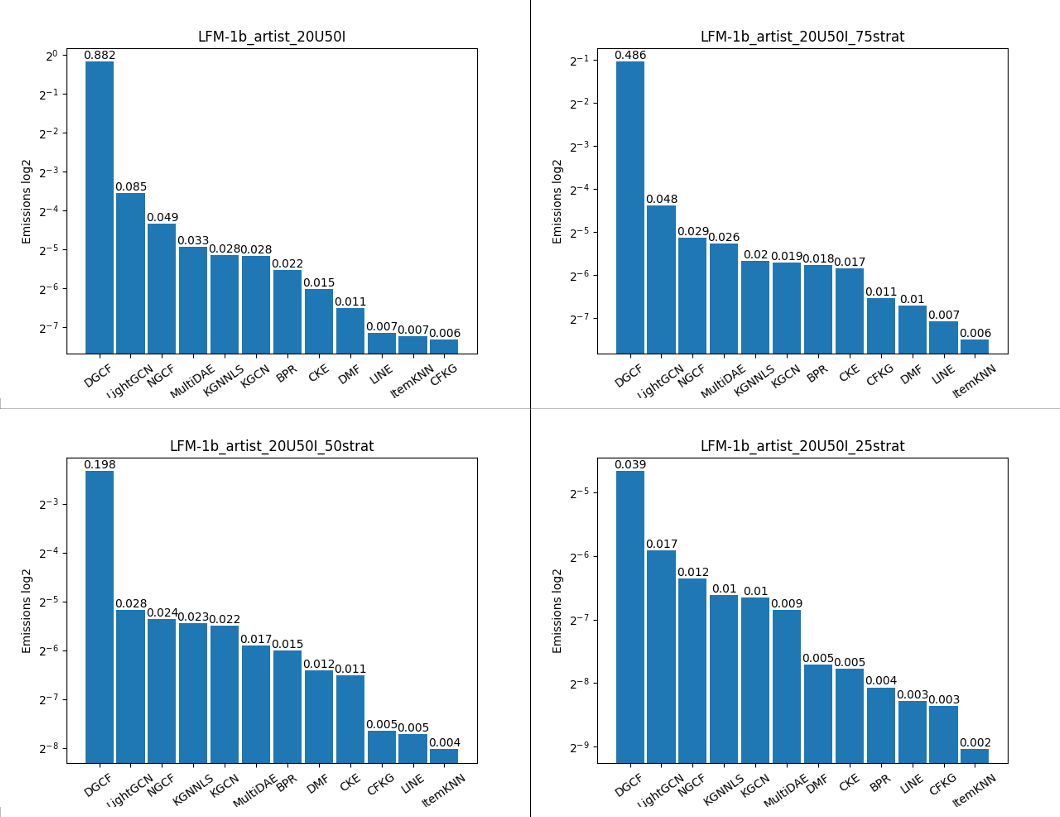
\includegraphics[width=\linewidth, trim=0 0 0 0]{images/EmissioniLFM.png} & 
            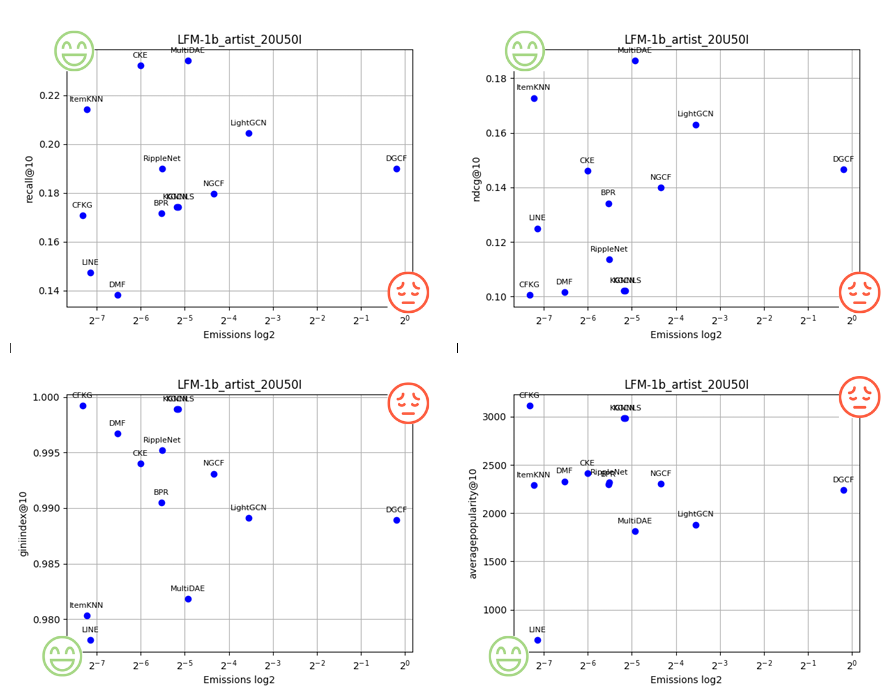
\includegraphics[width=\linewidth, trim=0 0 0 0]{images/TradeOff.png} \\
            \hline
        \end{tabularx}
        \caption{Emissioni di CO2 per i vari modelli e trade-off tra emissioni e performance}
    \end{table}
\end{frame}


\begin{frame}{RQ2 Addestramento sostenibile - Introduzione}
    \begin{wrapfigure}{r}{0.6\textwidth}
        \centering
        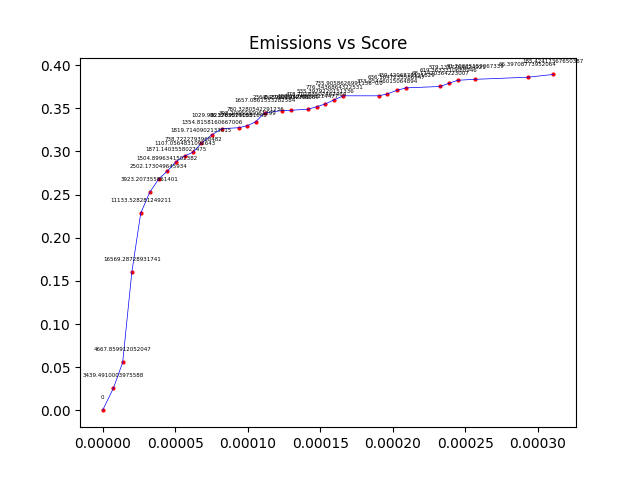
\includegraphics[width=0.6\textwidth, height=0.6\textheight]{images/curve_emissions_score.png}
        \caption{Andamento score e emissioni}
    \end{wrapfigure} 
Sull'asse delle x troviamo le emissioni, sull'asse delle y lo score. Quando la derivata è al di sotto di una certa soglia \textbf{S} per un certo numero di epoche consecutive \textbf{E} l'addestramento termina (comportamento asintotico).
Approssimazione della derivata della curva:
\begin{equation*}
    \frac{f(x_{i+1}) - f(x_i)}{x_{i+1} - x_i}
\end{equation*}
\end{frame}



\begin{frame}{RQ2 Addestramento sostenibile - Esplorazione}
    \begin{table}[H]
        \centering
        \resizebox{\textwidth}{!}{
        \begin{tabular}{|c|c|c|c|c|}
            \hline
            \textbf{Modello} & \textbf{Emissioni criterio classico (g)} & \textbf{Emissioni criterio nuovo (g)} & \textbf{Riduzione} & \textbf{\% riduzione emissioni} \\
            \hline
            DMF & 2.2927 & 1.97 & 0.32 & 14.21 \\
            \hline
            LINE & 1.91 & 1.38 & 0.53 & 27.69 \\
            \hline
            NGCF & 7.76 & 2.66 & 5.09 & 65.71 \\
            \hline
            DGCF & 94.90 & 10.46 & 84.44 & 88.97 \\
            \hline
        \end{tabular}
        }
        \caption{Esempi di confronto emissioni}
    \end{table}

    \begin{table}[H]
        \centering
        \resizebox{\textwidth}{!}{
            \begin{tabular}{|c|c|c|c|c|c|}
                \hline
                \textbf{Metrica} & \textbf{Modello} & \textbf{Score criterio classico} & \textbf{Score criterio nuovo} & \textbf{Riduzione} & \textbf{\% riduzione score} \\
                \hline
                \multirow{4}{*}{recall@10}
                                             & DMF & 0.14 & 0.14 & 0.0 & 0.0 \\ \cline{2-6}
                                             & LINE & 0.15 & 0.15 & 0.0 & 0.0 \\ \cline{2-6}
                                             & NGCF & 0.15 & 0.14 & 0.01 & 6.67 \\ \cline{2-6}
                                             & DGCF & 0.17 & 0.10 & 0.07 & 41.18 \\ \cline{2-6}
                \hline
            \end{tabular}
        }
        \caption{Esempi di confronto score}
        \label{tab:confronto-score}
    \end{table}
\end{frame}


\begin{comment}
\begin{frame}{RQ2 Addestramento sostenibile - Esplorazione}
 \begin{figure}[H]
    \centering
    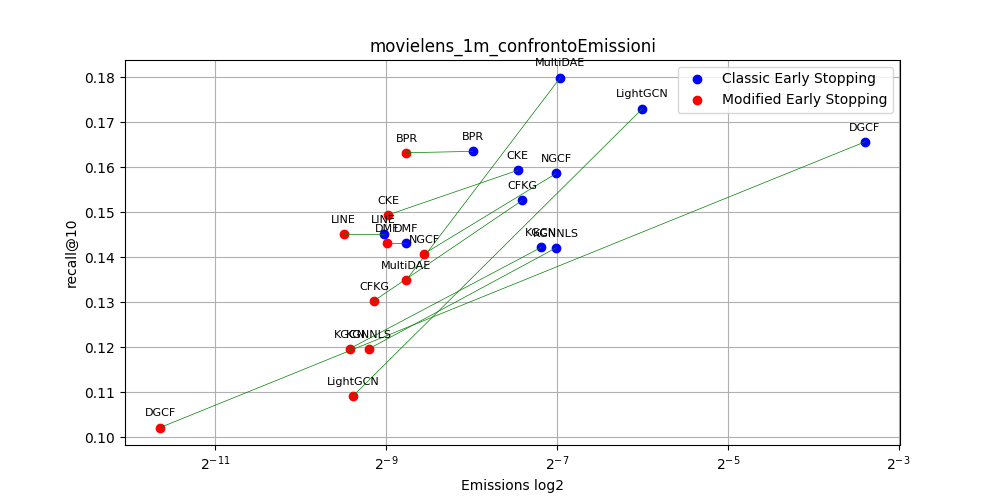
\includegraphics[scale=0.5]{images/recall@10_movielens_1m_comparison.png}
 \end{figure}
\end{frame}
\end{comment}



\begin{frame}{RQ3 Addestramento sostenibile - Confronto criteri}
    Sono stati eseguiti diversi esperimenti sul dataset MovieLens1M per confrontare diverse configurazioni dei parametri di soglia e di epoche, di seguito alcuni esempi\\
    \begin{table}[H]
        \centering
        \begin{tabular}{|c|c|c|c|}
            \hline
            \textbf{Modello} & \textbf{(Soglia,Epoche)} & \textbf{Riduzione emissioni} & \textbf{Riduzione score recall@10} \\ \hline
            \multirow{2}{*}{DMF} & (40,5) & 0.30 & 0 \\ \cline{2-4}
                                 & (30,7) &  0.31 & 0 \\ \hline
            \multirow{2}{*}{LINE} & (40,5) & 0.48 & 0 \\ \cline{2-4}
                                  & (30,7) & 0.47 & 0 \\ \hline
            \multirow{2}{*}{NGCF} & (40,5) & 5.0 & 0.02 \\ \cline{2-4}
                                  & (30,7) &  4.63 & 0.01 \\ \hline
            \multirow{2}{*}{DGCF} & (40,5) & 84.48 & 0.06 \\ \cline{2-4}
                                  & (30,7) & 81.52 &  0.05 \\ \hline
        \end{tabular}
        \caption{Esempi di risultati ottenuti}
    \end{table}
\end{frame}


\begin{frame}{RQ3 Addestramento sostenibile - Risultati confronto criteri}
\begin{table}[H]
    \scriptsize
    \centering
    \begin{tabular}{|c|c|c|}
        \hline
        \textbf{Modello} & \textbf{Parametro più impattante} & \textbf{Migliori risultati} \\
        \hline
        BPR & Soglia & Soglia 40 e 6 epoche \\
        \hline
        CFKG & Soglia & Soglia 40 e 6 epoche \\
        \hline
        CKE & Epoche consecutive & Soglia 40 e 6 epoche \\
        \hline
        DMF & Nessuno predominante & Soglia 40 e 7 epoche \\
        \hline
        KGCN & Epoche consecutive & Soglia 40 e 5 epoche \\
        \hline
        KGNNLS & Soglia & Soglia 40 e 5 epoche \\
        \hline
        LINE & Soglia & Soglia 40 e 7 epoche \\
        \hline
        MultiDAE & Soglia & Soglia 40 e 7 epoche \\
        \hline
        LightGCN & Soglia & Soglia 40 e 6 epoche \\
        \hline
        NGCF & Epoche consecutive & Soglia 40 e 5 epoche \\
        \hline
        DGCF & Epoche consecutive & Soglia 40 e 6 epoche \\
        \hline
    \end{tabular}
    \caption{Parametri più impattanti e migliori risultati per ciascun modello}
\end{table}
\end{frame}


\begin{frame}{RQ3 Addestramento sostenibile - Risultati confronto criteri}
\begin{table}[H]
    \scriptsize
    \centering
        \begin{tabular}{|c|c|c|c|}
            \hline
            \textbf{Tipo di Modello} & \textbf{Parametro predominante} & \textbf{Numero di Modelli} & \textbf{Modelli} \\ \hline
            Collaborative Filtering & Soglia & 5 & BPR, DMF, LightGCN, MultiDAE, LINE \\ \hline
            Collaborative Filtering & Epoche & 2 & NGCF, DGCF \\ \hline
            Knowledge Aware & Soglia & 2 & CFKG, KGNNLS \\ \hline
            Knowledge Aware & Epoche & 2 & CKE, KGCN \\ \hline
        \end{tabular}
    \caption{Riassunto dei parametri dominanti per tipo di modello}
\end{table}

\end{frame}
\section{Conclusioni e sviluppi futuri}
\subsection{Conclusioni}
Vengono qui brevemente riassunti i risultati ottenuti e le conclusioni a cui si è giunti in seguito al lavoro svolto.
\begin{itemize}
    \item \textbf{Benchmarking}: Vengono confermate le ipotesi iniziali per cui modelli più complessi emettono molta più CO2 rispetto a modelli più semplici senza però ottenere un miglioramento significativo delle metriche di valutazione (a volte addirittura peggiori). Si può notare inoltre come alcuni modelli tendono ad avere performance simili con qualsiasi dataset, mentre altri variano molto in base al dataset utilizzato.
    \item \textbf{Lavoro sul regressore}: Il regressore proposto ha ottenuto risultati peggiori rispetto al lavoro iniziale. Il dataset a disposizione sicuramente risulta essere più grande e vario nelle feature di input rispetto a quello utilizzato inizialmente, ma risultata essere molto sbilanciato nella feature di output in quando ci sono modelli che, a prescindere dal dataset, svettano rispetto agli altri in emissioni di molto e ciò ha portato il regressore a non riuscire a generalizzare bene
    \item \textbf{Addestramento sostenibile}: Il lavoro svolto ha portato a risultati interessanti. Si è dimostrato che è possibile addestrare un modello di Recommender System in maniera sostenibile, riducendo le emissioni di CO2 rispetto all'addestramento standard mantenendo però delle performance accettabili. Sono anche stati individuati dei pattern che possono aiutare a comprendere quali parametri del criterio di early stopping influenzino maggiormente l'addestramento in determinati contesti.
\end{itemize}
\subsection{Sviluppi futuri}
Il lavoro svolto ha dunque sicuramente mosso dei passi in avanti in ambito Recommender Systems e sostenibilità ambientale, ma siamo solo agli inizi. Ci sono diverse direzioni in cui si potrebbe andare per migliorare il sistema proposto:
\begin{itemize}
    \item \textbf{Benchmarking}: E' necessario effettuare più esperimenti variando i dataset, i modelli ma sopratutto l'hardware su cui si effettuano gli addestramenti. Questo permetterebbe di avere una visione più chiara delle prestazioni in relazione alle emissioni di CO2.
    \item \textbf{Lavoro sul regressore}: Con molti più dati a disposizione il regressore potrebbe essere addestrato su un dataset più grande e più vario. Inoltre, si potrebbero provare diverse architetture di rete neurale (oltre ai classici regressori), altri regressori e lavorare su diversi iperparametri per cercare di ottenere un modello più accurato.
    \item \textbf{Addestramento sostenibile}: Anche in questo caso variare dataset, modelli, hardware e parametri di early stopping (soglia e epoche consecutive) potrebbe portare a risultati interessanti che potrebbero confermare o smentire le ipotesi fatte in questo lavoro.
    \item \textbf{Lavorare sugli iperparametri}: Gli esperimenti effettuati in questo lavoro sono stati effettuati con i parametri di default. Gli stessi esperimenti (Benchmarking, regressore e addestramento sostenibile) potrebbero essere ripetuti con la ricerca degli iperparametri migliori per ogni modello e confrontare poi con i risultati ottenuti con i parametri di default. In questo modo si potrebbe vedere se le emissioni emesse per la ricerca degli iperparametri sono giustificate dai risultati ottenuti (quindi elevati miglioramenti).
\end{itemize}
\finalpagetext{Grazie per l'attenzione!}
\makefinalpage
\end{document}